\section{Coverage of numerical solutions for serial and parallel algorithms} \label{s:appendix:coverage-of-numerical-solutions}
	\begin{figure}[!htbp]
		\centering
		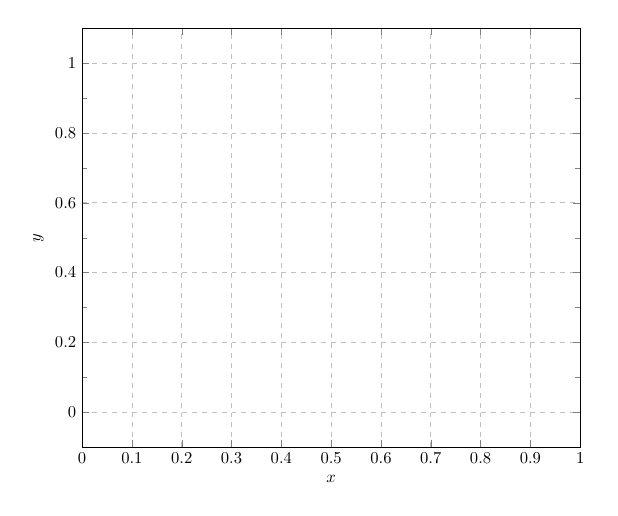
\begin{tikzpicture}[scale=0.6]	 	
			\pgfplotsset{width=\textwidth}
			\begin{axis}[
				xlabel = {$x$},
				ylabel = {$y$},
				%ymin = -1, ymax = 1,
				xmin = 5, xmax = 13,
				minor y tick num = 1,
				ymajorgrids=true,
				xmajorgrids=true,
				grid style=dashed,
				legend pos=north east
				]		
				\addcustomplot{others/comparison-num-analytic/implicit-upwind-serial-chart.csv}{red}{2}{Analytical}
				\addcustomplotblank{others/comparison-num-analytic/implicit-upwind-serial-chart.csv}{blue}{1}{Serial}{4}	 		\addcustomplot{others/comparison-num-analytic/implicit-upwind-parallel-chart.csv}{green}{1}{Parallel}
			\end{axis}
		\end{tikzpicture}
		\caption{Numerical solution comparison using implicit upwind scheme for serial and parallel algorithms. $\gls{CFL} = 0.01$ and $10000$ grid points.}
		\label{fig:comparison:implicit-upwind}
	\end{figure}

	\begin{figure}[!htbp]
		\centering
		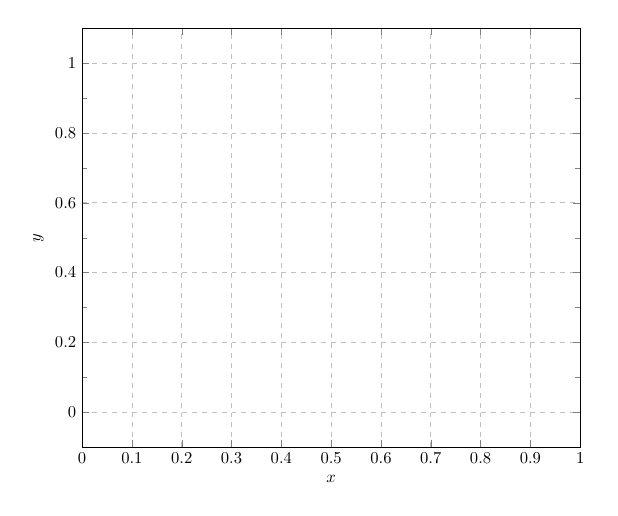
\begin{tikzpicture}[scale=0.6]	 	
		\pgfplotsset{width=\textwidth}
			\begin{axis}[
				xlabel = {$x$},
				ylabel = {$y$},
				%ymin = -1, ymax = 1,
				xmin = 5, xmax = 13,
				minor y tick num = 1,
				ymajorgrids=true,
				xmajorgrids=true,
				grid style=dashed,
				legend pos=north east
				]		
				\addcustomplotblank{others/comparison-num-analytic/explicit-upwind-serial-chart.csv}{red}{2}{Analytical}{6}
				\addcustomplotblank{others/comparison-num-analytic/explicit-upwind-serial-chart.csv}{blue}{1}{Serial}{4}	 		\addcustomplot{others/comparison-num-analytic/explicit-upwind-parallel-chart.csv}{green}{1}{Parallel}
			\end{axis}
		\end{tikzpicture}
		\caption{Numerical solution comparison using explicit upwind scheme for serial and parallel algorithms. $\gls{CFL} = 0.99$ and $10000$ grid points.}
		\label{fig:comparison:explicit-upwind}
	\end{figure}

	\begin{figure}[!htbp]
		\centering
		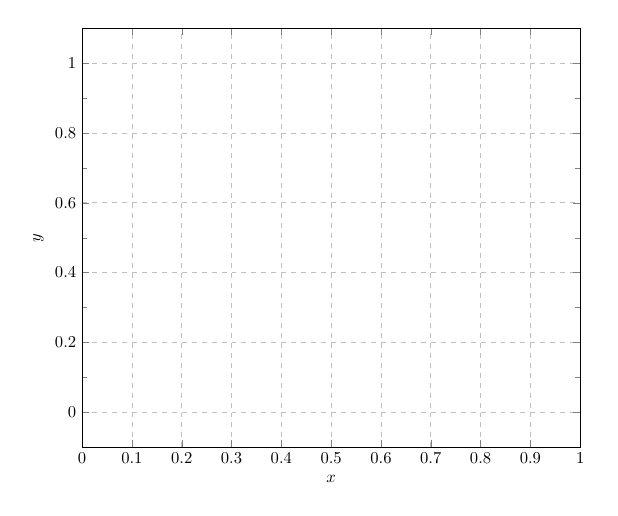
\begin{tikzpicture}[scale=0.6]	 	
			\pgfplotsset{width=\textwidth}
			\begin{axis}[
				xlabel = {$x$},
				ylabel = {$y$},
				%ymin = -1, ymax = 1,
				xmin = 5, xmax = 13,
				minor y tick num = 1,
				ymajorgrids=true,
				xmajorgrids=true,
				grid style=dashed,
				legend pos=north east
				]		
				\addcustomplotblank{others/comparison-num-analytic/crank-nicolson-serial-chart.csv}{red}{2}{Analytical}{6}
				\addcustomplotblank{others/comparison-num-analytic/crank-nicolson-serial-chart.csv}{blue}{1}{Serial}{4}	 		\addcustomplot{others/comparison-num-analytic/crank-nicolson-parallel-chart.csv}{green}{1}{Parallel}
			\end{axis}
		\end{tikzpicture}
		\caption{Numerical solution comparison using Crank-Nicolson scheme for serial and parallel algorithms. $\gls{CFL} = 0.1$ and $10000$ grid points.}
		\label{fig:comparison:crank-nicsolson}
	\end{figure}